\chapter{The Poincar\'{e} Conjecture}
\label{ch:poincare}

\noindent\textbf{Key Ideas.}
\begin{itemize}
  \item A \emph{manifold}\index{manifold} is a space that locally looks like Euclidean space.
  \item The \emph{fundamental group}\index{fundamental group} detects holes by tracking how loops can be deformed.
  \item The Poincar\'{e} conjecture\index{Poincaré conjecture} asks: does trivial topology force a 3-manifold to be the 3-sphere?
  \item The proof uses the \emph{Ricci flow}\index{Ricci flow}---a PDE that evolves geometry to become uniform.
\end{itemize}

\bigskip

\section{Introduction}

The Poincar\'{e} conjecture is one of the most famous problems in mathematics. It is the only one of the seven Millennium Prize Problems to have been solved, and its solver---Grigori Perelman\index{Perelman}---turned down both the Fields Medal and the one-million-dollar prize.

In this chapter, we will develop the mathematical background needed to understand the conjecture, trace its history from Henri Poincar\'{e}'s original 1904 question to Perelman's 2002--2003 proof, and explore the human drama surrounding the solution. The story spans a century of mathematics, connecting topology, geometry, and analysis in unexpected ways.

The conjecture asks a deceptively simple question: \emph{if a three-dimensional space has no holes, must it be a three-sphere?} In two dimensions, the answer is yes: a closed surface without holes is a sphere. Poincar\'{e} asked whether this holds in three dimensions. The answer turned out to be yes, but proving it required a revolution in geometric analysis.

\begin{quote}
\textbf{Informal statement.} If you can stretch, bend, and deform a 3D shape without tearing it, and it has no ``holes''---must it be a sphere?
\end{quote}

The difficulty is that in three dimensions, our geometric intuition fails. There exist strange spaces that \emph{look} like $S^3$ from the perspective of loops and surfaces, but are not $S^3$. Detecting and ruling out these imposters is what makes the problem hard.

\section{Topological Preliminaries}

Before we can state the conjecture, we need to understand what a manifold is.

\begin{definition}
An \textit{$n$-dimensional topological manifold}\index{topological manifold} is a second-countable Hausdorff topological space $M$ such that every point has a neighborhood homeomorphic to $\mathbb{R}^n$ or the closed half-space $\mathbb{R}^n_{\ge 0} = \{(x_1, \ldots, x_n) : x_n \ge 0\}$.
\end{definition}

Points with a neighborhood homeomorphic to $\mathbb{R}^n_{\ge 0}$ but not to $\mathbb{R}^n$ form the \textit{boundary} $\partial M$. If $\partial M = \emptyset$, we say $M$ is a \textit{closed manifold} if it is also compact.

\begin{example}
The \textit{$n$-sphere}\index{sphere} $S^n = \{x \in \mathbb{R}^{n+1} : \|x\| = 1\}$ is a compact $n$-manifold without boundary.
\end{example}

\begin{example}
The \textit{$n$-torus}\index{torus} $T^n = S^1 \times \cdots \times S^1$ (product of $n$ circles) is a compact $n$-manifold.
\end{example}

\begin{example}
The \textit{real projective plane} $\mathbb{RP}^2$ is the set of lines through the origin in $\mathbb{R}^3$. It is a compact 2-manifold that cannot be embedded in $\mathbb{R}^3$ without self-intersection.
\end{example}

\begin{example}[A non-manifold]
A figure-eight is \emph{not} a manifold. At the crossing point, no neighborhood looks like $\mathbb{R}^1$---instead, four branches meet at a single point. Manifolds must look ``the same'' at every point, locally.
\end{example}

\begin{checkyou}
Which of the following are 2-manifolds? (a) A triangle (boundary of a 2-simplex), (b) a Möbius band\index{Möbius band}, (c) two circles joined at a point.
\end{checkyou}

\begin{definition}
Two spaces $X$ and $Y$ are \textit{homeomorphic}\index{homeomorphism} if there exists a continuous bijection $f: X \to Y$ with a continuous inverse. A homeomorphism preserves all topological properties.
\end{definition}

\begin{remark}
Two spaces are homeomorphic if one can be continuously deformed into the other without cutting or gluing. A coffee cup is homeomorphic to a doughnut. A sphere is \emph{not} homeomorphic to a torus.
\end{remark}

\begin{definition}
A space $X$ is \textit{contractible} if the identity map $\mathrm{id}_X$ is homotopic to a constant map.
\end{definition}

\begin{definition}
A space $X$ is \textit{simply connected}\index{simply connected} if it is path-connected and its fundamental group $\pi_1(X)$ is trivial.
\end{definition}

\begin{example}[The 2-sphere is simply connected]
\label{ex:s2simplyconnected}
We show that every loop on $S^2$ can be contracted to a point, proving $\pi_1(S^2) = 0$.

\textbf{Setup.} Let $\gamma: [0,1] \to S^2$ be an arbitrary loop based at $p \in S^2$, so $\gamma(0) = \gamma(1) = p$.

\textbf{Step 1: Reduce to a contractible case via stereographic projection.}
Since $S^2 \subset \mathbb{R}^3$, the image $\gamma([0,1])$ is a compact subset of $S^2$. By a dimension argument, $\gamma$ cannot be surjective: a continuous image of a 1-dimensional domain cannot cover a 2-dimensional manifold. Choose a point $q \in S^2$ not in the image of $\gamma$. The stereographic projection from $q$ is a homeomorphism:
\[
\sigma_q: S^2 \setminus \{q\} \;\xrightarrow{\;\sim\;}\; \mathbb{R}^2
\]
Since $\gamma$ never visits $q$, we may view $\gamma$ as a loop in $\mathbb{R}^2$.

\textbf{Step 2: Contract in $\mathbb{R}^2$.}
The space $\mathbb{R}^2$ is contractible. Define the straight-line homotopy $H: [0,1] \times [0,1] \to \mathbb{R}^2$ by:
\[
H(t, s) = (1 - s)\,\gamma(t) + s \cdot \sigma_q(p)
\]
At $s = 0$: $H(t,0) = \gamma(t)$ (the original loop). At $s = 1$: $H(t,1) = \sigma_q(p)$, a constant loop. For all $s$: $H(0,s) = H(1,s) = \sigma_q(p)$ (the basepoint is fixed). Each $H(\cdot, s)$ is continuous and its image lies in $\mathbb{R}^2$, which is convex, so $H$ is well-defined.

\textbf{Step 3: Transfer back to $S^2$.}
The map $\sigma_q^{-1}: \mathbb{R}^2 \to S^2 \setminus \{q\}$ is a homeomorphism. Define the homotopy on $S^2$:
\[
\widetilde{H}(t, s) = \sigma_q^{-1}\bigl(H(t, s)\bigr)
\]
This is a continuous deformation of $\gamma$ to the constant loop at $p$, lying entirely on $S^2$. Therefore $\gamma \simeq \mathrm{const}_p$, and since $\gamma$ was arbitrary, $\pi_1(S^2) = 0$. The 2-sphere is simply connected.
\end{example}

\subsection{The Fundamental Group}

In 1895, Henri Poincar\'{e}\index{Poincaré, Henri} introduced a powerful algebraic tool for studying manifolds: the fundamental group.

\begin{quote}
\textbf{Intuition.} Imagine the manifold is made of rubber. The fundamental group asks: which loops can be continuously shrunk to a point? If every loop can be shrunk, the space is simply connected (``no holes''). If some loops cannot be shrunk, the fundamental group records how they ``wrap around'' the holes.
\end{quote}

\begin{definition}
Let $X$ be a topological space with basepoint $x_0 \in X$. A \textit{loop} based at $x_0$ is a continuous map $\gamma: [0, 1] \to X$ with $\gamma(0) = \gamma(1) = x_0$. Two loops $\gamma_0, \gamma_1$ are \textit{homotopic} (written $\gamma_0 \simeq \gamma_1$) if there exists a continuous map $H: [0, 1] \times [0, 1] \to X$ such that $H(t, 0) = \gamma_0(t)$, $H(t, 1) = \gamma_1(t)$, and $H(0, s) = H(1, s) = x_0$ for all $t, s$.
\end{definition}

The set of homotopy classes of loops forms a group under concatenation:
\[
[\gamma_1] \cdot [\gamma_2] = [\gamma_1 \circ \gamma_2]
\]
where $\gamma_1 \circ \gamma_2$ means ``traverse $\gamma_1$ first, then $\gamma_2$.''

\begin{definition}
The \textit{fundamental group} $\pi_1(X, x_0)$ is the group of homotopy classes of loops based at $x_0$ with the concatenation operation.
\end{definition}

\begin{example}[$\pi_1(S^1) \cong \mathbb{Z}$ via the covering space $\mathbb{R} \to S^1$]
\label{ex:pi1s1}
We compute the fundamental group of the circle by lifting loops to its universal cover.

\textbf{The covering map.} Define $p: \mathbb{R} \to S^1$ by $p(t) = e^{2\pi i t} = (\cos 2\pi t,\, \sin 2\pi t)$. This is a covering map: every point of $S^1$ has an open neighborhood $U$ whose preimage $p^{-1}(U)$ is a disjoint union of open intervals in $\mathbb{R}$, each mapped homeomorphically onto $U$ by $p$.

\textbf{Step 1: Lifting loops.}
Let $\gamma: [0,1] \to S^1$ be a loop based at $1 \in S^1$, so $\gamma(0) = \gamma(1) = 1$. By the \textit{lifting property} of covering spaces, there exists a unique continuous lift $\tilde{\gamma}: [0,1] \to \mathbb{R}$ satisfying $p \circ \tilde{\gamma} = \gamma$ and $\tilde{\gamma}(0) = 0$.

Since $p(\tilde{\gamma}(1)) = \gamma(1) = 1 = p(0)$, we have $\tilde{\gamma}(1) \in p^{-1}(1) = \mathbb{Z}$. Define the \textit{winding number}:
\[
w(\gamma) = \tilde{\gamma}(1) \in \mathbb{Z}
\]
This is the integer that records how many times $\gamma$ winds around $S^1$.

\textbf{Step 2: Homotopic loops have the same winding number.}
Suppose $\gamma_0 \simeq \gamma_1$ via a homotopy $H: [0,1] \times [0,1] \to S^1$ fixing the basepoint. Lift $H$ to $\widetilde{H}: [0,1] \times [0,1] \to \mathbb{R}$ with $\widetilde{H}(t,0) = \tilde{\gamma}_0(t)$ and $\widetilde{H}(0,s) = 0$ for all $s$. Since $\widetilde{H}(1,s) \in \mathbb{Z}$ for each $s$ and $s \mapsto \widetilde{H}(1,s)$ is continuous, it must be constant (a continuous integer-valued function on a connected set is constant). Therefore $w(\gamma_0) = \widetilde{H}(1,0) = \widetilde{H}(1,1) = w(\gamma_1)$.

\textbf{Step 3: Every integer is realized.}
For any $k \in \mathbb{Z}$, the loop $\gamma_k(t) = e^{2\pi i k t}$ winds around $S^1$ exactly $k$ times. Its lift is $\tilde{\gamma}_k(t) = kt$, so $w(\gamma_k) = k$.

\textbf{Step 4: Winding number classifies loops up to homotopy.}
We must show that if $w(\gamma_0) = w(\gamma_1) = k$, then $\gamma_0 \simeq \gamma_1$. Since $w(\gamma_j) = k$, the lifts $\tilde{\gamma}_j$ both start at $0$ and end at $k$. Define:
\[
\widetilde{H}(t, s) = (1-s)\,\tilde{\gamma}_0(t) + s\,\tilde{\gamma}_1(t)
\]
This is a straight-line homotopy in $\mathbb{R}$ from $\tilde{\gamma}_0$ to $\tilde{\gamma}_1$. Since $\mathbb{R}$ is convex, $\widetilde{H}$ is continuous. Moreover, $\widetilde{H}(0,s) = 0$ and $\widetilde{H}(1,s) = k$ for all $s$, so the basepoint is fixed. Projecting down: $H = p \circ \widetilde{H}$ is a homotopy in $S^1$ from $\gamma_0$ to $\gamma_1$.

\textbf{Conclusion.} The map $w: \pi_1(S^1) \to \mathbb{Z}$ is a well-defined, surjective bijection. It is a group homomorphism (winding numbers add under loop concatenation), hence an isomorphism: $\pi_1(S^1) \cong \mathbb{Z}$.
\end{example}

For path-connected spaces, $\pi_1(X, x_0) \cong \pi_1(X, x_1)$ for any two basepoints, so we often write $\pi_1(X)$.

\begin{example}
$\pi_1(S^n) = 0$ for $n \ge 2$. On the $2$-sphere, any loop can be contracted to a point. Think of a rubber band on a basketball: you can always slide it off.
\end{example}

\begin{example}
$\pi_1(S^1) \cong \mathbb{Z}$. The nontrivial loops wrap around the circle $k$ times. This is why a rubber band around a cylinder cannot be contracted---it wraps around the hole.
\end{example}

\begin{example}
$\pi_1(T^2) \cong \mathbb{Z} \times \mathbb{Z}$, generated by loops around each independent circle direction.
\end{example}

\begin{example}
$\pi_1(\mathbb{R}^n) = 0$ for all $n$, since $\mathbb{R}^n$ is contractible---any loop can be pulled to a point.
\end{example}

\begin{checkyou}
Why is the fundamental group of a figure-eight (two circles joined at a point) the free group on two generators, while the fundamental group of a circle is $\mathbb{Z}$?
\end{checkyou}

\begin{definition}
A space $X$ is \textit{simply connected} if it is path-connected and $\pi_1(X)$ is the trivial group.
\end{definition}

\begin{checkyou}
Is $\mathbb{R}^n$ simply connected? What about $\mathbb{R}^n \setminus \{0\}$? Why or why not?
\end{checkyou}

\subsection{Higher Homotopy Groups}

The fundamental group is only the first in a sequence of homotopy groups $\pi_n(X)$ for $n \ge 1$. The $n$-th homotopy group consists of homotopy classes of maps $S^n \to X$. A theorem of Hurewicz relates homotopy groups to homology groups, which are often easier to compute.

\begin{theorem}[Hurewicz Theorem]
If $X$ is simply connected, then the first nontrivial homotopy group $\pi_n(X)$ is isomorphic to the first nontrivial homology group $H_n(X)$.
\end{theorem}

\subsection{Homology and Cohomology}

While homotopy groups capture information about maps from spheres, homology groups capture information about cycles and boundaries in a space.

\begin{definition}
For a topological space $X$, the \textit{singular homology groups} $H_n(X; \mathbb{Z})$ are abelian groups that count $n$-dimensional ``holes'' in $X$. The $n$-th Betti number\index{Betti numbers} is $b_n = \mathrm{rank}(H_n(X; \mathbb{Z}))$.
\end{definition}

\begin{example}
For $S^n$: $H_0(S^n) = \mathbb{Z}$, $H_n(S^n) = \mathbb{Z}$, and $H_k(S^n) = 0$ for $0 < k < n$.
\end{example}

\begin{example}
For $T^n$: $H_k(T^n) = \mathbb{Z}^{\binom{n}{k}}$.
\end{example}

\subsection{The Classification of Surfaces}

Before attacking three-dimensional manifolds, mathematicians classified all compact 2-manifolds (surfaces)\index{surface}. The theorem is elegant:

\begin{theorem}[Classification of compact surfaces]
Every closed, connected, orientable 2-manifold\index{orientable} is homeomorphic to a sphere with $g$ handles ($g \ge 0$), called the \textit{genus-$g$ surface} $\Sigma_g$. The number $g$ is called the \textit{genus}\index{genus}. Non-orientable surfaces are homeomorphic to connected sums of $\mathbb{RP}^2$'s.
\end{theorem}

In particular, a simply connected closed surface must be the 2-sphere $S^2$. This is the 2-dimensional analogue of the Poincar\'{e} conjecture.

\begin{figure}[htbp]
\centering
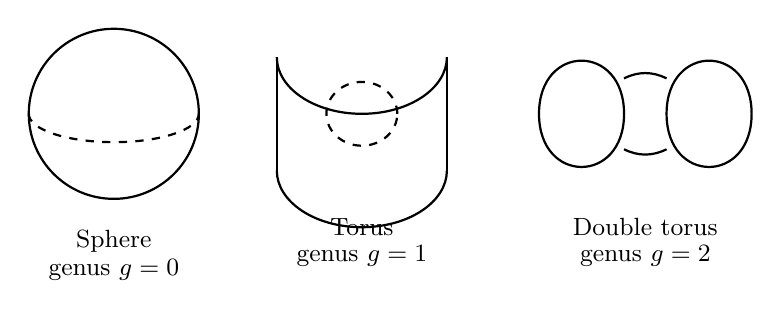
\begin{tikzpicture}[scale=0.9]
  % Sphere (genus 0)
  \begin{scope}[xshift=-3.5cm]
    \draw[thick] (0,0) circle (1.2);
    \draw[thick,dashed] (-1.2,0) arc[start angle=180, end angle=360, x radius=1.2, y radius=0.4];
    \node at (0,-1.8) {\small Sphere};
    \node at (0,-2.2) {\small genus $g=0$};
  \end{scope}
  % Torus (genus 1)
  \begin{scope}[xshift=0cm]
    \draw[thick] (-1.2,-0.8) arc[start angle=180, end angle=360, x radius=1.2, y radius=0.8];
    \draw[thick] (-1.2,0.8) arc[start angle=180, end angle=360, x radius=1.2, y radius=0.8];
    \draw[thick] (-1.2,-0.8) -- (-1.2,0.8);
    \draw[thick] (1.2,-0.8) -- (1.2,0.8);
    \draw[thick,dashed] (0,0) ellipse[x radius=0.5, y radius=0.45];
    \node at (0,-1.6) {\small Torus};
    \node at (0,-2.0) {\small genus $g=1$};
  \end{scope}
  % Genus-2 surface
  \begin{scope}[xshift=4cm]
    \draw[thick] (-1.5,0) .. controls (-1.5,1.0) and (-0.3,1.0) .. (-0.3,0);
    \draw[thick] (-0.3,0) .. controls (-0.3,-1.0) and (-1.5,-1.0) .. (-1.5,0);
    \draw[thick] (0.3,0) .. controls (0.3,1.0) and (1.5,1.0) .. (1.5,0);
    \draw[thick] (1.5,0) .. controls (1.5,-1.0) and (0.3,-1.0) .. (0.3,0);
    \draw[thick] (-0.3,0.5) .. controls (-0.1,0.6) and (0.1,0.6) .. (0.3,0.5);
    \draw[thick] (-0.3,-0.5) .. controls (-0.1,-0.6) and (0.1,-0.6) .. (0.3,-0.5);
    \node at (0,-1.6) {\small Double torus};
    \node at (0,-2.0) {\small genus $g=2$};
  \end{scope}
\end{tikzpicture}
\caption{The classification of surfaces by genus: every closed orientable surface is homeomorphic to a sphere with $g$ handles.}
\label{fig:surfaces}
\end{figure}

\subsection{Connected Sum and Prime Decomposition}

For 3-manifolds, there is an analogous operation to the connected sum of surfaces.

\begin{definition}
The \textit{connected sum} $M \# N$ of two $n$-manifolds is formed by removing an $n$-ball from each and gluing the resulting boundaries.
\end{definition}

\begin{theorem}[Prime decomposition, Kneser 1929; uniqueness, Milnor 1962]
Every closed, orientable 3-manifold can be uniquely decomposed as a connected sum of \textit{prime} 3-manifolds (manifolds that cannot be written as a nontrivial connected sum).
\end{theorem}

The Poincar\'{e} conjecture is equivalent to: every simply connected prime 3-manifold is $S^3$.

\section{Statement of the Conjecture}

The Poincar\'{e} conjecture asks whether the analogous statement holds in three dimensions:

\begin{theorem}[Poincar\'{e} conjecture, now proved]
Every simply connected, closed 3-manifold is homeomorphic to the 3-sphere\index{three-sphere} $S^3$.
\end{theorem}

\begin{remark}
The 3-sphere is the set $\{(x_1, x_2, x_3, x_4) \in \mathbb{R}^4 : x_1^2 + x_2^2 + x_3^2 + x_4^2 = 1\}$. It is the natural generalization of an ordinary sphere to one dimension higher.
\end{remark}

\begin{figure}[htbp]
\centering
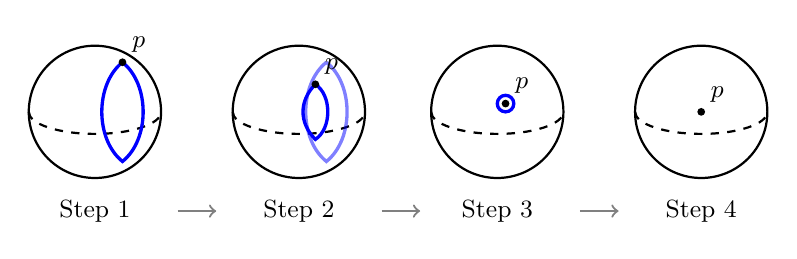
\begin{tikzpicture}[scale=0.7]
  % Step 1: loop on sphere
  \begin{scope}[xshift=-5.5cm]
    \draw[thick] (0,0) circle (1.2);
    \draw[thick,dashed] (-1.2,0) arc[start angle=180, end angle=360, x radius=1.2, y radius=0.4];
    \draw[blue,very thick] (0.5,0.9) .. controls (1.0,0.5) and (1.0,-0.5) .. (0.5,-0.9)
      .. controls (0.0,-0.5) and (0.0,0.5) .. (0.5,0.9);
    \fill (0.5,0.9) circle (2pt) node[above right] {\small $p$};
  \end{scope}
  % Step 2: loop shrinking
  \begin{scope}[xshift=-1.8cm]
    \draw[thick] (0,0) circle (1.2);
    \draw[thick,dashed] (-1.2,0) arc[start angle=180, end angle=360, x radius=1.2, y radius=0.4];
    \draw[blue,very thick,opacity=0.5] (0.5,0.9) .. controls (1.0,0.5) and (1.0,-0.5) .. (0.5,-0.9)
      .. controls (0.0,-0.5) and (0.0,0.5) .. (0.5,0.9);
    \draw[blue,very thick] (0.3,0.5) .. controls (0.6,0.3) and (0.6,-0.3) .. (0.3,-0.5)
      .. controls (0.0,-0.2) and (0.0,0.2) .. (0.3,0.5);
    \fill (0.3,0.5) circle (2pt) node[above right] {\small $p$};
  \end{scope}
  % Step 3: loop almost a point
  \begin{scope}[xshift=1.8cm]
    \draw[thick] (0,0) circle (1.2);
    \draw[thick,dashed] (-1.2,0) arc[start angle=180, end angle=360, x radius=1.2, y radius=0.4];
    \draw[blue,very thick] (0.15,0.15) circle (0.15);
    \fill (0.15,0.15) circle (2pt) node[above right] {\small $p$};
  \end{scope}
  % Step 4: contracted to point
  \begin{scope}[xshift=5.5cm]
    \draw[thick] (0,0) circle (1.2);
    \draw[thick,dashed] (-1.2,0) arc[start angle=180, end angle=360, x radius=1.2, y radius=0.4];
    \fill (0,0) circle (2pt) node[above right] {\small $p$};
  \end{scope}
  % Labels below each sphere
  \node at (-5.5,-1.8) {\small Step 1};
  \node at (-1.8,-1.8) {\small Step 2};
  \node at (1.8,-1.8) {\small Step 3};
  \node at (5.5,-1.8) {\small Step 4};
  % Arrows between steps
  \draw[->,thick,gray] (-4.0,-1.8) -- (-3.3,-1.8);
  \draw[->,thick,gray] (-0.3,-1.8) -- (0.4,-1.8);
  \draw[->,thick,gray] (3.3,-1.8) -- (4.0,-1.8);
\end{tikzpicture}
\caption{Any loop on a simply connected surface (such as $S^2$) can be continuously contracted to a point. This is the property that the Poincar\'{e} conjecture seeks to generalize to three dimensions.}
\label{fig:loop_contraction}
\end{figure}

\begin{remark}
The analogue holds in all dimensions $\ge 5$ (proved by Stephen Smale in 1961, Fields Medal 1966) and in dimension 4 (proved by Michael Freedman in 1982, Fields Medal 1986). Dimension 3 was the hardest case.
\end{remark}

\subsection{The Poincar\'{e} Conjecture in Higher Dimensions}

It is worth understanding why dimensions $\ge 5$ were easier. The key technique is the \textit{h-cobordism theorem} and \textit{surgery theory}\index{surgery theory}.

\begin{theorem}[Smale's h-cobordism theorem]
Let $W$ be a compact $(n+1)$-manifold with boundary $\partial W = M_0 \cup M_1$, where $M_0$ and $M_1$ are $n$-manifolds. If $n \ge 5$ and $W$, $M_0$, $M_1$ are simply connected, and the inclusion $M_0 \hookrightarrow W$ is a homotopy equivalence\index{homotopy equivalence}, then $W$ is diffeomorphic to $M_0 \times [0,1]$.
\end{theorem}

This theorem allows one to build a cobordism between a homotopy sphere and the standard sphere, and then conclude they are diffeomorphic. The proof requires the \textit{Whitney trick} to eliminate intersections of disks, which works in dimensions $\ge 5$ but fails in dimensions 3 and 4.

In dimension 4, Freedman's proof used topological (not smooth) methods and the \textit{Casson handle} construction, which is an infinite tower of disks that substitutes for the Whitney trick.

\subsection{Historical Formulations}

Poincar\'{e} originally stated the conjecture in 1904 in the fifth supplement to his \textit{Analysis Situs}:

\begin{quote}
``Une question se pose: Est-il possible que le groupe fondamental d'une vari\'{e}t\'{e} de trois dimensions soit r\'{e}duit \`{a} l'identit\'{e} sans que cette vari\'{e}t\'{e} soit simplement connexe? ... Je ne suis pas parvenu \`{a} r\'{e}soudre cette question.''
\end{quote}

(A question arises: Is it possible that the fundamental group of a 3-dimensional manifold could be reduced to the identity without the manifold being simply connected? ... I have not succeeded in solving this question.)

He later modified the question to ask whether every closed 3-manifold with trivial fundamental group is homeomorphic to $S^3$. The conjecture in its modern form was thus established.

\section{Hamilton's Program: The Ricci Flow}

The key to proving the Poincar\'{e} conjecture was the \textit{Ricci flow}, introduced by Richard Hamilton\index{Hamilton} in 1982.

\begin{quote}
\textbf{Intuition.} The Ricci flow is the ``heat equation for geometry.'' Just as heat spreads out from hot spots to make temperature uniform, the Ricci flow smooths out the curvature of a manifold to make it round. If you start with any 3-manifold and flow, the geometry should eventually look like a sphere.
\end{quote}

\begin{definition}
Let $(M, g)$ be a Riemannian manifold with metric $g_{ij}$. The \textit{Ricci flow} is the evolution equation:
\[
\frac{\partial}{\partial t} g_{ij} = -2 R_{ij}
\]
where $R_{ij}$ is the Ricci curvature tensor.
\end{definition}

\begin{checkyou}
In what sense is the Ricci flow like the heat equation? What plays the role of ``temperature''?
\end{checkyou}

The Ricci curvature $R_{ij}$ measures how the volume of a small ball deviates from Euclidean volume. Regions of positive Ricci curvature shrink under the flow; regions of negative Ricci curvature expand.

Think of the Ricci flow as the geometric analogue of the heat equation. Just as heat diffuses from hot regions to cold regions, the Ricci flow smooths out irregularities in the metric, making the geometry more uniform over time.

\subsection{The Heat Analogy}

The ordinary heat equation $\partial_t u = \Delta u$ describes how temperature diffuses. A hot object eventually reaches uniform temperature. Similarly, under the Ricci flow, a manifold with positive Ricci curvature should evolve toward a round sphere---the 3-sphere.

Hamilton showed that in dimension 2, the Ricci flow does indeed deform any metric on a closed surface to a constant-curvature metric, providing a new proof of the uniformization theorem. He also showed that in dimension 3, if the Ricci flow can be continued indefinitely without developing singularities, it would prove the Poincar\'{e} conjecture.

\begin{figure}[htbp]
\centering
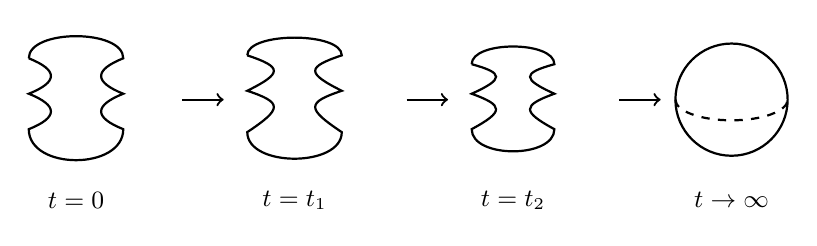
\begin{tikzpicture}[scale=0.75]
  % Dumbbell shape evolving under Ricci flow (Hamilton's picture)
  % Stage 1: pinched dumbbell
  \begin{scope}[xshift=-5.5cm]
    \draw[thick] (-0.8,0.7) .. controls (-0.8,1.2) and (0.8,1.2) .. (0.8,0.7)
      .. controls (0.3,0.5) and (0.3,0.3) .. (0.8,0.1)
      .. controls (0.3,-0.1) and (0.3,-0.3) .. (0.8,-0.5)
      .. controls (0.8,-1.2) and (-0.8,-1.2) .. (-0.8,-0.5)
      .. controls (-0.3,-0.3) and (-0.3,-0.1) .. (-0.8,0.1)
      .. controls (-0.3,0.3) and (-0.3,0.5) .. (-0.8,0.7);
    \node at (0,-1.7) {\small $t=0$};
  \end{scope}
  % Stage 2: slightly less pinched
  \begin{scope}[xshift=-1.8cm]
    \draw[thick] (-0.8,0.75) .. controls (-0.8,1.15) and (0.8,1.15) .. (0.8,0.75)
      .. controls (0.2,0.55) and (0.2,0.45) .. (0.8,0.15)
      .. controls (0.2,-0.05) and (0.2,-0.15) .. (0.8,-0.55)
      .. controls (0.8,-1.15) and (-0.8,-1.15) .. (-0.8,-0.55)
      .. controls (-0.2,-0.15) and (-0.2,-0.05) .. (-0.8,0.15)
      .. controls (-0.2,0.45) and (-0.2,0.55) .. (-0.8,0.75);
    \node at (0,-1.7) {\small $t=t_1$};
  \end{scope}
  % Stage 3: rounding out
  \begin{scope}[xshift=1.9cm]
    \draw[thick] (-0.7,0.6) .. controls (-0.7,1.0) and (0.7,1.0) .. (0.7,0.6)
      .. controls (0.15,0.45) and (0.15,0.35) .. (0.7,0.1)
      .. controls (0.15,-0.1) and (0.15,-0.2) .. (0.7,-0.5)
      .. controls (0.7,-1.0) and (-0.7,-1.0) .. (-0.7,-0.5)
      .. controls (-0.15,-0.2) and (-0.15,-0.1) .. (-0.7,0.1)
      .. controls (-0.15,0.35) and (-0.15,0.45) .. (-0.7,0.6);
    \node at (0,-1.7) {\small $t=t_2$};
  \end{scope}
  % Stage 4: nearly round
  \begin{scope}[xshift=5.6cm]
    \draw[thick] (0,0) circle (0.95);
    \draw[thick,dashed] (-0.95,0) arc[start angle=180, end angle=360, x radius=0.95, y radius=0.35];
    \node at (0,-1.7) {\small $t \to \infty$};
  \end{scope}
  % Arrows
  \draw[->,thick] (-3.7,0) -- (-3.0,0);
  \draw[->,thick] (0.1,0) -- (0.8,0);
  \draw[->,thick] (3.7,0) -- (4.4,0);
\end{tikzpicture}
\caption{The Ricci flow smooths out irregularities in curvature, analogous to heat diffusion. A ``dumbbell'' shape with a thin neck (high curvature) evolves toward a round sphere. The thin neck pinches off and the geometry becomes uniform.}
\label{fig:ricci_flow_dumbbell}
\end{figure}

\subsection{The Singularity Problem}

The obstacle that stymied Hamilton was the formation of \textit{singularities}. As the flow evolves a 3-manifold, regions of extreme curvature can develop, causing the flow to break down. Imagine a rubber band being stretched until it snaps---that is analogous to a singularity.

Hamilton identified several possible singularity types and developed a program for handling them:
\begin{enumerate}
  \item Understand the possible singularity models
  \item Show that certain bad singularities do not occur
  \item When singularities occur, perform ``surgery'' to remove them
  \item Show that after finitely many surgeries, the manifold decomposes into pieces with uniform geometry
\end{enumerate}

He was unable to complete steps 1--3.

\subsection{Hamilton's Results}

Hamilton made remarkable progress:
\begin{itemize}
  \item Short-time existence and uniqueness for Ricci flow on compact manifolds
  \item In dimension 2: Ricci flow converges to constant curvature metric (uniformization)
  \item In dimension 3: if initial metric has positive Ricci curvature, the flow exists for all time and converges to round sphere
  \item Development of the maximum principle for systems of PDEs on manifolds
  \item Introduction of the differential Harnack inequality for Ricci flow
\end{itemize}

But the general case with arbitrary initial metrics remained out of reach.

\section{Perelman's Breakthrough}

Grigori Perelman, working alone in Saint Petersburg, made three key contributions that completed Hamilton's program.

\subsection{1. The Entropy Functional}

In his first paper (November 2002), Perelman introduced the $\mathcal{F}$ and $\mathcal{W}$ functionals. The $\mathcal{W}$ functional, which he called the \textit{entropy}\index{entropy}, is:

\[
\mathcal{W}(g, f, \tau) = \int_M \bigl[\tau(|\nabla f|^2 + R) + f - n\bigr] (4\pi\tau)^{-n/2} e^{-f} \, dV
\]

where $f$ is a smooth function on $M$ and $\tau > 0$ is a parameter.

\begin{theorem}[Perelman, 2002]
The $\mathcal{W}$ functional is monotone non-decreasing under the Ricci flow coupled with a certain evolution equation for $f$. Moreover, $\mathcal{W}$ is bounded below.
\end{theorem}

This monotonicity gave Perelman unprecedented control over the formation of singularities. He used it to show that singularities must be of a very specific type: they must be \textit{asymptotically cylindrical} or \textit{asymptotically paraboloidal}. In particular, singularities cannot accumulate.

\subsection{2. No Local Collapsing Theorem}

A second crucial result: Perelman showed that the Ricci flow cannot develop a singularity where the geometry collapses to arbitrarily small scales---he called this \textit{no local collapsing}. This ruled out certain pathological singularity types that Hamilton could not exclude.

\begin{theorem}[Perelman, No Local Collapsing]
Under the Ricci flow on a closed 3-manifold, there is no sequence of points and scales where the injectivity radius tends to zero while the curvature remains bounded.
\end{theorem}

The proof uses the $\mathcal{W}$ entropy and a clever scaling argument.

\subsection{3. Ricci Flow with Surgery}

In his second paper (March 2003), Perelman described an explicit surgical procedure. When a singularity begins to form (the curvature becomes large in a small region), he showed how to cut out the singular region and replace it with a smooth cap. The surgery can be performed at a precise curvature threshold, and the procedure can be repeated.

\begin{theorem}[Perelman, 2003]
For any initial metric on a closed 3-manifold, the Ricci flow with surgery can be continued for all time, with only finitely many surgeries occurring.
\end{theorem}

The third paper (July 2003) proved that after finitely many surgeries, all remaining components are diffeomorphic to spherical space forms or $S^2 \times S^1$, and for a simply connected manifold, only a single $S^3$ remains.

\subsection{The Canonical Neighborhood Theorem}

A key technical result in Perelman's work is the \textit{canonical neighborhood theorem}, which classifies the geometry of high-curvature regions. Every point of sufficiently high curvature has a neighborhood that is, after rescaling, close to one of a few model geometries:
\begin{itemize}
  \item A neck region (approximately $S^2 \times \mathbb{R}$)
  \item A cap region (approximately a capped cylinder)
  \item A component that is globally close to a spherical space form
\end{itemize}

This classification makes surgery possible: one cuts along the necks and caps the ends.

\subsection{Finite Extinction Time}

Perelman also proved that for any initial metric on a simply connected 3-manifold, the Ricci flow with surgery becomes extinct in finite time---meaning the manifold disappears entirely, having been completely decomposed into spherical space forms. This is a stronger result than just proving the Poincar\'{e} conjecture.

\begin{checkyou}
Why does finite extinction time imply the Poincar\'{e} conjecture for simply connected manifolds?
\end{checkyou}

\section{Verification and Acceptance}

Perelman posted his papers on the arXiv preprint server rather than submitting them to journals. The mathematical community faced the challenge of verifying his work:

\begin{itemize}
  \item \textbf{2003:} Perelman visited the US to lecture at MIT, Princeton, Stony Brook, and Columbia.
  \item \textbf{2003--2006:} Bruce Kleiner and John Lott wrote detailed notes.
  \item \textbf{2004--2006:} John Morgan and Gang Tian wrote a comprehensive exposition.
  \item \textbf{2006:} The International Mathematical Union awarded Perelman the Fields Medal.
  \item \textbf{2010:} The Clay Mathematics Institute awarded the Millennium Prize.
\end{itemize}

Perelman declined both awards. He told a journalist: ``I'm not interested in money or fame. I don't want to be on display like an animal in a zoo.''

\subsection{The Verification Efforts}

Three major teams worked on verifying Perelman's proof:
\begin{enumerate}
  \item \textbf{Kleiner--Lott:} Detailed notes on all three papers, published in \textit{Geometry \& Topology} (2008).
  \item \textbf{Morgan--Tian:} Book-length exposition \textit{Ricci Flow and the Poincar\'{e} Conjecture} (AMS, 2007).
  \item \textbf{Cao--Zhu:} Published in \textit{Asian Journal of Mathematics} (2006), though later controversy arose about attribution.
\end{enumerate}

All three teams confirmed the correctness of Perelman's arguments. The mathematical community reached consensus that the Poincar\'{e} conjecture was proved.

\section{The Thurston Geometrization Conjecture}

Perelman's proof actually accomplished far more than the Poincar\'{e} conjecture. He proved the \textit{Thurston geometrization conjecture}\index{Thurston's geometrization}, which classifies \textit{all} 3-manifolds.

\begin{theorem}[Thurston geometrization, proved by Perelman]
Every closed 3-manifold can be decomposed along spheres and tori into pieces that admit one of eight geometric structures (the eight Thurston geometries): $S^3$, $\mathbb{E}^3$, $\mathbb{H}^3$, $S^2 \times \mathbb{R}$, $\mathbb{H}^2 \times \mathbb{R}$, $\widetilde{SL_2(\mathbb{R})}$, $\mathrm{Nil}$, and $\mathrm{Sol}$.
\end{theorem}

This is analogous to the classification of surfaces, but vastly richer and more complex.

\subsection{The Eight Thurston Geometries}

The eight model geometries for 3-manifolds are:
\begin{enumerate}
  \item \textbf{Spherical ($S^3$):} Positive constant curvature. Compact.
  \item \textbf{Euclidean ($\mathbb{E}^3$):} Zero curvature. Flat.
  \item \textbf{Hyperbolic ($\mathbb{H}^3$):} Negative constant curvature. Most 3-manifolds are hyperbolic.
  \item \textbf{$S^2 \times \mathbb{R}$:} Product of sphere and line.
  \item \textbf{$\mathbb{H}^2 \times \mathbb{R}$:} Product of hyperbolic plane and line.
  \item \textbf{$\widetilde{SL_2(\mathbb{R})}$}: Universal cover of the unit tangent bundle of $\mathbb{H}^2$.
  \item \textbf{Nil}: Nilpotent Lie group (Heisenberg group).
  \item \textbf{Sol}: Solvable Lie group.
\end{enumerate}

Every closed 3-manifold admits a unique decomposition (the \textit{geometric decomposition}) into pieces that have one of these geometries.

\subsection{The Poincar\'{e} Conjecture as a Special Case}

The Poincar\'{e} conjecture follows immediately: a simply connected closed 3-manifold must be a spherical space form. The only simply connected spherical space form is $S^3$ itself.

\section{The Human Story}

The solution of the Poincar\'{e} conjecture involves one of the most remarkable human stories in modern mathematics.

\subsection{Grigori Perelman}

Grigori Perelman (born 1966) was a child prodigy in Leningrad. He won a gold medal with a perfect score at the 1982 International Mathematical Olympiad. He received his Ph.D. from Leningrad State University under the direction of Aleksandr Aleksandrov. He worked at the Steklov Institute in Saint Petersburg.

In 1992--1993, Perelman spent time in the US at NYU, SUNY Stony Brook, and UC Berkeley. Colleagues remember him as intensely focused, living ascetically, and completely dedicated to mathematics. He returned to Saint Petersburg and worked in isolation for seven years before posting his papers.

\subsection{The Controversies}

The verification process was not without controversy:
\begin{itemize}
  \item The Cao--Zhu paper initially claimed credit for ``completing'' Perelman's work, leading to protests from the mathematical community.
  \item Perelman was offered the Fields Medal in 2006 at the International Congress of Mathematicians in Madrid. He declined, and did not attend.
  \item The Clay Institute awarded the Millennium Prize in 2010. Perelman declined the prize money, saying his contribution was no greater than Hamilton's.
  \item Perelman resigned from the Steklov Institute in 2005 and has reportedly not done mathematics since.
\end{itemize}

\subsection{Richard Hamilton}

Richard Hamilton (born 1943) developed the Ricci flow program over two decades. He proved the foundational results and guided the program to the point where Perelman could complete it. Hamilton received the Shaw Prize in 2011 and the AMS Steele Prize in 2009. He has been gracious in acknowledging Perelman's achievement.

\subsection{William Thurston}

William Thurston (1946--2012) formulated the geometrization conjecture in the 1970s. His visionary insight was that 3-manifolds should be understood through geometry. He received the Fields Medal in 1982. Perelman's proof realized Thurston's vision.

\section{The Ricci Flow in Higher Dimensions}

The Ricci flow has been extensively studied in higher dimensions since Perelman's work.

\begin{itemize}
  \item \textbf{Dimension 4:} The Ricci flow with surgery is more complicated due to the presence of \textit{orbifold} singularities and the lack of a canonical neighborhood theorem as clean as in dimension 3. Recent work by Bamler, Kleiner, and others has made progress.
  \item \textbf{K\"{a}hler-Ricci flow:} On K\"{a}hler manifolds, the Ricci flow preserves the K\"{a}hler condition. This has applications to the classification of algebraic varieties (the Minimal Model Program).
  \item \textbf{Ancient solutions:} Classification of ancient solutions (solutions existing for all negative time) is a major area of study.
\end{itemize}

\section{Applications and Legacy}

The resolution of the Poincar\'{e} conjecture has had far-reaching consequences:

\subsection{Geometric Topology}
\begin{itemize}
  \item Complete classification of 3-manifolds (geometrization)
  \item Solution to the homeomorphism problem for 3-manifolds
  \item Understanding of the mapping class groups of 3-manifolds
\end{itemize}

\subsection{Geometric Analysis}
\begin{itemize}
  \item New techniques for nonlinear PDE on manifolds (entropy, pseudolocality, surgery)
  \item Development of the theory of Ricci flow as a field in its own right
  \item Applications to the differentiable sphere theorem (Brendle-Schoen, 2008)
\end{itemize}

\subsection{Physics}
\begin{itemize}
  \item Ricci flow as renormalization group flow in string theory
  \item Connections to the AdS/CFT correspondence
  \item Understanding of topology change in quantum gravity
\end{itemize}

\section{Exercises}

\begin{exercise}
Show that $S^2$ is simply connected by constructing an explicit homotopy contracting any loop to a point.
\end{exercise}

\begin{exercise}
Compute $\pi_1(\mathbb{R}^2 \setminus \{0\})$.
\end{exercise}

\begin{exercise}
Show that the fundamental group of the figure-eight space (two circles joined at a point) is the free group on two generators.
\end{exercise}

\begin{exercise}
Explain in your own words why the Ricci flow analogy with the heat equation is useful. What are the key differences?
\end{exercise}

\begin{exercise}
Research the proof of the 2-dimensional analogue: why is every simply connected closed surface homeomorphic to $S^2$?
\end{exercise}

\begin{exercise}
The Poincar\'{e} conjecture in dimension 5 and higher was proved by Smale using surgery theory. Write a one-page summary of how surgery works.
\end{exercise}

\begin{exercise}
\textbf{Challenge problem.} A \textit{Hopf fibration} is a map $h: S^3 \to S^2$ whose fibers are circles. Show that $S^3$ can be described as the union of two solid tori glued along their boundaries. Use this to compute $\pi_1(S^3)$.
\end{exercise}

\begin{exercise}
Let $M$ be a closed 3-manifold with $\pi_1(M) = 0$. Show that $H_1(M; \mathbb{Z}) = 0$ and $H_2(M; \mathbb{Z}) = 0$. (Hint: use the Hurewicz theorem and Poincar\'{e} duality.)
\end{exercise}

\begin{exercise}
Explain the difference between a topological manifold, a smooth manifold, and a PL (piecewise-linear) manifold. Why did the Poincar\'{e} conjecture hold in all three categories in dimension 3?
\end{exercise}

\begin{exercise}
The \textit{Poincar\'{e} homology sphere} is a 3-manifold with the same homology as $S^3$ but with fundamental group of order 120. Describe its construction as a quotient of $S^3$ by a finite group action.
\end{exercise}

\section{Further Reading}

\begin{itemize}
  \item J. Milnor, ``The Poincar\'{e} conjecture,'' official Clay problem description
  \item J. Morgan and G. Tian, \textit{Ricci Flow and the Poincar\'{e} Conjecture}, AMS, 2007
  \item A. Hatcher, \textit{Algebraic Topology}, Cambridge, 2002
  \item B. Kleiner and J. Lott, ``Notes on Perelman's papers,'' \textit{Geometry \& Topology}, 2008
  \item H.-D. Cao and X.-P. Zhu, ``A complete proof of the Poincar\'{e} and geometrization conjectures,'' \textit{Asian J. Math.}, 2006
  \item J. W. Morgan, ``Recent progress on the Poincar\'{e} conjecture and the classification of 3-manifolds,'' \textit{Bull. AMS}, 2005
  \item D. Anderson, ``The Poincar\'{e} conjecture,'' \textit{Notices AMS}, 2004
  \item G. Perelman, ``The entropy formula for the Ricci flow and its geometric applications,'' arXiv:math/0211159
  \item G. Perelman, ``Ricci flow with surgery on three-manifolds,'' arXiv:math/0303109
  \item G. Perelman, ``Finite extinction time for the solutions to the Ricci flow on certain three-manifolds,'' arXiv:math/0307245
\end{itemize}

\section*{Chapter Summary}

\noindent\textbf{What we learned:}
\begin{itemize}
  \item A \emph{topological manifold} is a space that locally resembles Euclidean space; the fundamental group $\pi_1(X)$ measures its ``loop structure.''
  \item The \emph{Poincar\'{e} conjecture} states that every simply connected closed 3-manifold is homeomorphic to $S^3$.
  \item The conjecture was proved by Perelman using \emph{Ricci flow with surgery}: evolve the metric to smooth out curvature, perform surgery at singularities, and show the manifold decomposes into spheres.
  \item Perelman's proof established the far stronger \emph{Thurston geometrization conjecture}, classifying all closed 3-manifolds.
\end{itemize}

\noindent\textbf{Key technique:} The Ricci flow $\partial_t g_{ij} = -2R_{ij}$ is a nonlinear PDE that evolves a Riemannian metric toward uniform curvature. The main difficulty---formation of singularities---was resolved by Perelman's entropy monotonicity and surgery procedure.

\noindent\textbf{Connections to other chapters:} The Ricci flow is a geometric PDE, connecting to the Navier--Stokes equations (Chapter~4) through the general theory of nonlinear evolution equations. The classification of 3-manifolds uses algebraic topology (fundamental groups, homology) that also appears in the Hodge conjecture (Chapter~6).